% Provenance (never printed): see sources/outline_sources.md (Year 3:
% speciation and saturation indices; carbonate equilibria applied to rocks;
% weathering kinetics; hydrothermal fluids). Brief: sources/book5/BRIEFS.md,
% ch. 15. Curves from figdata/bachelor-3/carbonate_system.py,
% activity_diagram.py, weathering_rates.py. Exercise and problem values in the
% Book 5 scratch calculator calc/ch15.py. The spring below the Varden
% limestone, its analysis and the granite stream are invented.
\chapter{Interação água--rocha}\label{ch:b3:water-rock-interaction}

Uma nascente ao pé de uma escarpa calcária deixa uma crosta branca em cada
galho e pedra que toca; um riacho que drena um granito carrega sílica, sódio
e um pouco de potássio, e não deixa crosta alguma. A diferença está na
química da água, e essa química é um registro da rocha que a água
atravessou: quanto dióxido de carbono ela carregou, quanto tempo permaneceu, quais
minerais dissolveu e quais construiu. Este capítulo lê esse registro com
as ferramentas da química de soluções, desde a análise de uma água até as taxas de
dissolução mineral e os traços isotópicos de fluidos quentes na crosta.

\begin{recall}
Atividade, coeficiente de atividade, força iônica, especiação, o produto de
solubilidade, alcalinidade, o estado de saturação $\Omega$, a lei de Henry, leis de
velocidade, a lei de Arrhenius, o estado de transição e o valor $\delta$ estão nos
volumes universitários de química. O intemperismo químico, a hidrólise de
silicatos, os minerais argilosos e a caulinita estão no volume do primeiro ano, no
capítulo sobre intemperismo e argilas; a lisoclina e a profundidade de compensação
de carbonato no capítulo sobre sedimentos carbonáticos, silicosos e evaporíticos. O
fluido hidrotermal está no volume do segundo ano, no capítulo sobre depósitos
minerais, e o termostato do intemperismo de silicatos no capítulo sobre o clima ao longo
do tempo geológico; a circulação hidrotermal está nos livros escolares.
\end{recall}

\section{A análise de uma água natural}\label{sec:b3:water-rock-interaction:analysis}

Uma análise de água lista os íons principais em miligramas por litro: cálcio,
magnésio, sódio e potássio; bicarbonato, cloreto, sulfato e nitrato;
sílica dissolvida como \ce{SiO2}; e o pH e a temperatura medidos na
nascente, já que ambos mudam assim que a amostra sai dela. Dividindo pela massa
molar, obtêm-se milimols por litro e, multiplicando pela carga,
miliequivalentes. Uma água diluída é eletricamente neutra, de modo que a soma dos
cátions deve igualar a soma dos ânions.

\begin{method}[Verificação de uma análise de água]\label{met:b3:water-rock-interaction:analysis}
\begin{enumerate}
\item converte-se cada concentração em \unit{mmol/L} e em \unit{meq/L};
\item somam-se os cátions e os ânions em \unit{meq/L};
\item calcula-se o erro de balanço de cargas $100\,(\sum\text{cát} -
  \sum\text{ân})/(\sum\text{cát} + \sum\text{ân})$, em por cento;
\item aceita-se a análise se o erro estiver dentro de 1 ou \qty{2}{\percent} para uma
  água de 250 a \qty{1000}{mg/L}, um pouco mais para uma mais diluída;
  caso contrário, procura-se um íon ausente ou um erro analítico.
\end{enumerate}
\end{method}
% ledger: hem85:charge-balance

A atividade de um íon é sua molalidade multiplicada pelo seu coeficiente de
atividade $\gamma$. Em águas naturais, $\gamma$ calcula-se a partir da força iônica $I =
\tfrac12\sum m_i z_i^2$ com a equação estendida de Debye--Hückel
\[
-\log\gamma_i = \frac{A z_i^2\sqrt I}{1 + B a_i\sqrt I},
\]
com $A = 0.5085$ e $B = 0.3281$ para água a \qty{25}{\celsius}, e um
diâmetro iônico $a_i$ em ångströms: 9 para \ce{H+}, 8 para \ce{Mg^2+}, 6 para
\ce{Ca^2+}, 5 para \ce{CO3^2-}, 4 para \ce{Na+}, \ce{HCO3-} e \ce{SO4^2-},
3 para \ce{K+}, \ce{Cl-}, \ce{OH-} e \ce{NO3-}. A equação vale até
cerca de \qty{0.1}{mol/L} de sais monovalentes, o que abrange rios e a maioria das
águas subterrâneas, mas não a água do mar ou salmouras. A temperatura altera $A$ apenas de
0.4883 a \qty{0}{\celsius} para 0.5425 a \qty{60}{\celsius}, de modo que os valores a
\qty{25}{\celsius} servem também para águas frias.
% ledger: hem85:debye-huckel

O carbono inorgânico de uma água se distribui entre o dióxido de carbono dissolvido
(escrito \ce{CO2} para a soma de \ce{CO2} e \ce{H2CO3}), bicarbonato e
carbonato, relacionados por
\[
K_1 = \frac{a_{\ce{HCO3-}}\,a_{\ce{H+}}}{a_{\ce{CO2}}}, \qquad
K_2 = \frac{a_{\ce{CO3^2-}}\,a_{\ce{H+}}}{a_{\ce{HCO3-}}}, \qquad
K_H = \frac{a_{\ce{CO2}}}{P_{\ce{CO2}}},
\]
com $\log K_1 = -6.35$, $\log K_2 = -10.33$ e $\log K_H = -1.47$ a
\qty{25}{\celsius}, e $-6.46$, $-10.49$ e $-1.27$ a \qty{10}{\celsius}
($P$ em atmosferas). Entre pH 6.4 e 10.3 domina o bicarbonato, e na
maioria das águas naturais a alcalinidade é quase toda bicarbonato. O pH
e o bicarbonato medidos então fornecem as outras duas espécies, e a pressão parcial de
dióxido de carbono com a qual a água estaria em equilíbrio.
% ledger: phreeqc:carbonate

\section{Saturação}\label{sec:b3:water-rock-interaction:saturation}

\begin{definition}[Índice de saturação]\label{def:b3:water-rock-interaction:si}
O \emph{índice de saturação (de um mineral)}\index{índice de saturação (de um mineral)}
de uma água é $\mathrm{SI} = \log(\mathrm{IAP}/K)$, em que IAP é
o produto de atividade iônica da água escrito como o produto de solubilidade
$K$ do mineral: $\mathrm{SI} = \log\Omega$.
\end{definition}

Uma água com $\mathrm{SI} < 0$ pode dissolver o mineral, e uma com
$\mathrm{SI} > 0$ pode precipitá-lo, e $\mathrm{SI} = 0$ corresponde ao equilíbrio.
Como a energia livre da reação de dissolução é $\Delta_r G = RT\ln\Omega
= 2.303\,RT\,\mathrm{SI}$, o índice de saturação também é uma medida da
força motriz, em unidades de $2.303\,RT$, cerca de \qty{5.7}{kJ/mol} a
\qty{25}{\celsius}. Para a calcita $\mathrm{IAP} = a_{\ce{Ca^2+}}
a_{\ce{CO3^2-}}$ e $\log K = -8.45$ a \qty{25}{\celsius}, $-8.35$ a
\qty{10}{\celsius}: a calcita é mais solúvel em água fria. Para o gesso, $\mathrm{SI} = \log(a_{\ce{Ca^2+}}a_{\ce{SO4^2-}}) + 4.55$;
para o quartzo, cuja dissolução fornece \ce{H4SiO4} neutro, $\mathrm{SI} = \log
a_{\ce{H4SiO4}} + 3.98$, e para a sílica amorfa a constante é 2.71
em vez de 3.98. Os índices medidos carregam uma incerteza de pelo menos $\pm0.1$,
e uma água com valor dentro de $\pm0.3$ de zero é considerada próxima do equilíbrio.
% ledger: phreeqc:carbonate, phreeqc:silicates, hem85:si

\section{Equilíbrios carbonáticos nas rochas}\label{sec:b3:water-rock-interaction:carbonate}

A calcita se dissolve em água carregada de dióxido de carbono, segundo a reação
\[
\ce{CaCO3 + CO2 + H2O <=> Ca^2+ + 2 HCO3-},
\qquad K = \frac{a_{\ce{Ca^2+}}\,a_{\ce{HCO3-}}^2}{P_{\ce{CO2}}}
= \frac{K_{\mathrm{cal}}K_1K_H}{K_2},
\]
com $\log K = -5.94$ a \qty{25}{\celsius} e $-5.59$ a \qty{10}{\celsius}.
Quanto se dissolve depende da origem do dióxido de carbono.

\begin{definition}[Sistemas carbonáticos aberto e fechado]\label{def:b3:water-rock-interaction:open-closed}
Uma água dissolve calcita em um \emph{sistema carbonático aberto}\index{sistema carbonático aberto}
quando permanece em contato com um gás de
$P_{\ce{CO2}}$ fixa, que repõe o dióxido de carbono consumido. Ela o faz em um
\emph{sistema carbonático fechado}\index{sistema carbonático fechado} quando foi carregada antes com dióxido de carbono e
em seguida isolada do gás, de modo que
o dióxido de carbono que retém é tudo o que pode usar.
\end{definition}

\begin{theorem}[Solubilidade da calcita, aberto e fechado]\label{thm:b3:water-rock-interaction:calcite}
Para uma água do tipo bicarbonato de cálcio, com $m$ a molalidade do cálcio,
\[
\text{aberto:}\quad m = \left(\frac{K\,P_{\ce{CO2}}}{4\gamma_{\ce{Ca^2+}}
\gamma_{\ce{HCO3-}}^2}\right)^{1/3};
\qquad
\text{fechado:}\quad 4\gamma_{\ce{Ca^2+}}\gamma_{\ce{HCO3-}}^2\,m^3 =
\frac{K_{\mathrm{cal}}K_1}{K_2}\,(C_0 - m),
\]
em que $C_0 = K_H P_{\ce{CO2}}$ é o dióxido de carbono incorporado antes
de o sistema ser fechado.
\end{theorem}

\begin{proof}
Entre pH 6.5 e 8.5, carbonato, \ce{H+} e \ce{OH-} são desprezíveis diante do
bicarbonato, de modo que o balanço de cargas é $2m = m_{\ce{HCO3-}}$. No caso aberto: $K = \gamma
_{\ce{Ca^2+}}m\,\gamma_{\ce{HCO3-}}^2(2m)^2/P_{\ce{CO2}}$, o que fornece a
raiz cúbica. No caso fechado: cada cálcio dissolvido consome um \ce{CO2}, logo $m_{\ce{CO2}}
= C_0 - m$ e $a_{\ce{Ca^2+}}a_{\ce{HCO3-}}^2/a_{\ce{CO2}} = K/K_H =
K_{\mathrm{cal}}K_1/K_2$ resulta na cúbica.
\end{proof}

No sistema aberto o cálcio cresce como a raiz cúbica de $P_{\ce{CO2}}$; no
sistema fechado ele é limitado por $C_0$, e o dióxido de carbono restante no
final, portanto a $P_{\ce{CO2}}$ final, é muito menor que no início. O ar do
solo contém de 10 a 100 vezes o dióxido de carbono da atmosfera, produzido pelas
raízes e pela decomposição da matéria vegetal, e as águas subterrâneas costumam apresentar
$P_{\ce{CO2}}$ entre $10^{-2.5}$ e $10^{-1}$ atmosfera. A água em
contato com calcita e ar contém apenas cerca de \qty{20}{mg/L} de cálcio; a chuva que
atinge um calcário através de um solo, ainda aberta ao gás do solo, pode dissolver
quatro ou cinco vezes mais. O carste é esculpido por esse dióxido de carbono do solo.
% ledger: hem85:pco2, phreeqc:carbonate

O caminho de volta é a desgaseificação. Uma nascente que emerge de um calcário carrega
a $P_{\ce{CO2}}$ do solo e da rocha, de dez a cem vezes a do
ar. Ao ar livre ela perde dióxido de carbono, o bicarbonato se transforma em
carbonato, o pH sobe e o índice de saturação aumenta mais de uma unidade,
como mostra o painel (b) da figura abaixo, para a nascente do
problema de fim de semana deste capítulo.
A calcita precipita no leito do riacho e sobre musgos e galhos: tufo de
fontes frias, travertino de fontes quentes. Nascentes que atravessam a rocha
rapidamente, em dias ou semanas, por condutos, costumam chegar à superfície
subsaturadas; as que percolam lentamente por ela durante meses emergem próximas
da saturação.
% ledger: hem85:pco2, usgsyvo:travertine

\begin{omfigure}
\begin{tikzpicture}
\begin{groupplot}[group style={group size=2 by 1, horizontal sep=1.6cm},
  omrecord, width=0.47\linewidth, height=0.42\linewidth, title style={font=\small},
  tick label style={font=\scriptsize}, label style={font=\small},
  legend style={font=\scriptsize, legend cell align=left}]
\nextgroupplot[title={(a) solubilidade da calcita},
  xlabel={$\log P_{\ce{CO2}}$ (atm)}, ylabel={cálcio dissolvido (\unit{mmol/L})},
  xmin=-3.5, xmax=-1, ymin=0, ymax=5.5, clip=false,
  xtick={-3.5,-3,-2.5,-2,-1.5,-1}, xticklabels={$-3.5$,$-3$,$-2.5$,$-2$,$-1.5$,$-1$},
  legend style={at={(0.14,0.97)}, anchor=north west}]
\addplot[draw=none, fill=black!6, forget plot] coordinates {(-2.5,0) (-2.5,5.5) (-1,5.5) (-1,0)} -- cycle;
% computed in figdata/bachelor-3/carbonate_system.py
\addplot[omDef, thick] table[x=logp, y=ca_open10] {figdata/out/bachelor-3-carbonate_system-solubility.dat};
\addlegendentry{aberto, \qty{10}{\celsius}}
\addplot[red!70!black, thick] table[x=logp, y=ca_open25] {figdata/out/bachelor-3-carbonate_system-solubility.dat};
\addlegendentry{aberto, \qty{25}{\celsius}}
\addplot[omDef, thick, densely dashed] table[x=logp, y=ca_closed10] {figdata/out/bachelor-3-carbonate_system-solubility.dat};
\addlegendentry{fechado, \qty{10}{\celsius}}
\addplot[red!70!black, thick, densely dashed] table[x=logp, y=ca_closed25] {figdata/out/bachelor-3-carbonate_system-solubility.dat};
\addlegendentry{fechado, \qty{25}{\celsius}}
\draw[black, densely dotted] (axis cs:-3.37,0) -- (axis cs:-3.37,5.5);
\node[font=\scriptsize, anchor=south] at (axis cs:-3.37,5.5) {ar};
\node[font=\scriptsize, anchor=north] at (axis cs:-1.4,5.45) {águas subterrâneas};
\nextgroupplot[title={(b) a desgaseificação da nascente},
  xlabel={$\log P_{\ce{CO2}}$ (atm)}, ylabel={índice de saturação da calcita},
  xmin=-3.5, xmax=-1.5, ymin=-0.2, ymax=1.9, x dir=reverse, clip=false,
  xtick={-3.5,-3,-2.5,-2,-1.5}, xticklabels={$-3.5$,$-3$,$-2.5$,$-2$,$-1.5$}]
% computed in figdata/bachelor-3/carbonate_system.py
\addplot[omDef, thick] table[x=logp, y=si] {figdata/out/bachelor-3-carbonate_system-degassing.dat};
\addplot[black, densely dotted, domain=-3.5:-1.5, samples=2] {0};
\addplot[red!70!black, only marks, mark=*, mark size=1.6pt] table[x=logp, y=si] {figdata/out/bachelor-3-carbonate_system-ends.dat};
\node[font=\scriptsize, anchor=north west] at (axis cs:-1.84,-0.01) {saída};
\node[font=\scriptsize, anchor=north west] at (axis cs:-3.3,1.55) {ar};
\end{groupplot}
\end{tikzpicture}

\par\smallskip{\small (a) Cálcio dissolvido por água em equilíbrio com
calcita, em função da pressão parcial de dióxido de carbono (para o sistema
fechado, a pressão com que a água foi carregada): sistema aberto em linha contínua, sistema
fechado tracejado; a água fria dissolve mais; a faixa cinza é o intervalo de
águas subterrâneas. (b) A nascente abaixo do calcário Varden, a \qty{10}{\celsius},
perdendo dióxido de carbono na descida pela encosta (lido da esquerda para a direita, em eixo invertido)
antes de qualquer calcita se formar: seu cálcio e sua alcalinidade são fixos, seu pH sobe
de 7.2 para 8.8, e seu índice de saturação de 0.04 para 1.6. Constantes de
equilíbrio de um banco de dados público, coeficientes de atividade de Debye--Hückel
estendida.}\label{fig:b3:water-rock-interaction:calcite}
\end{omfigure}
% ledger: phreeqc:carbonate, hem85:debye-huckel, hem85:pco2, data:co2-mlo

A mesma química, executada na escala do oceano, aparece nos
volumes universitários dos livros de química; a profundidade em que a água do mar
se torna subsaturada em calcita, a lisoclina, e a profundidade abaixo da qual a calcita não
se acumula estão no volume do primeiro ano.

\begin{inthefield}[Uma nascente que constrói os próprios terraços]
\begin{minipage}[t]{0.52\linewidth}\vspace{0pt}
Na Palette Spring, uma das Mammoth Hot Springs do planalto de Yellowstone,
a água termal sobe através de um calcário soterrado e o carrega
dissolvido para longe. Na superfície, a água
se espalha sobre os próprios depósitos e perde dióxido de carbono, e o carbonato de cálcio
precipita como travertino, primeiro na borda de cada poça, onde a água é
mais rasa. Geólogos que levantam essas nascentes medem uma deposição de cerca de
três milímetros por dia, quinze vezes a taxa das tufas de
nascentes frias. As faixas laranja e
marrom são tapetes de micróbios amantes do calor que vivem no escoamento superficial quente.
\end{minipage}\hfill
\begin{minipage}[t]{0.44\linewidth}\vspace{0pt}
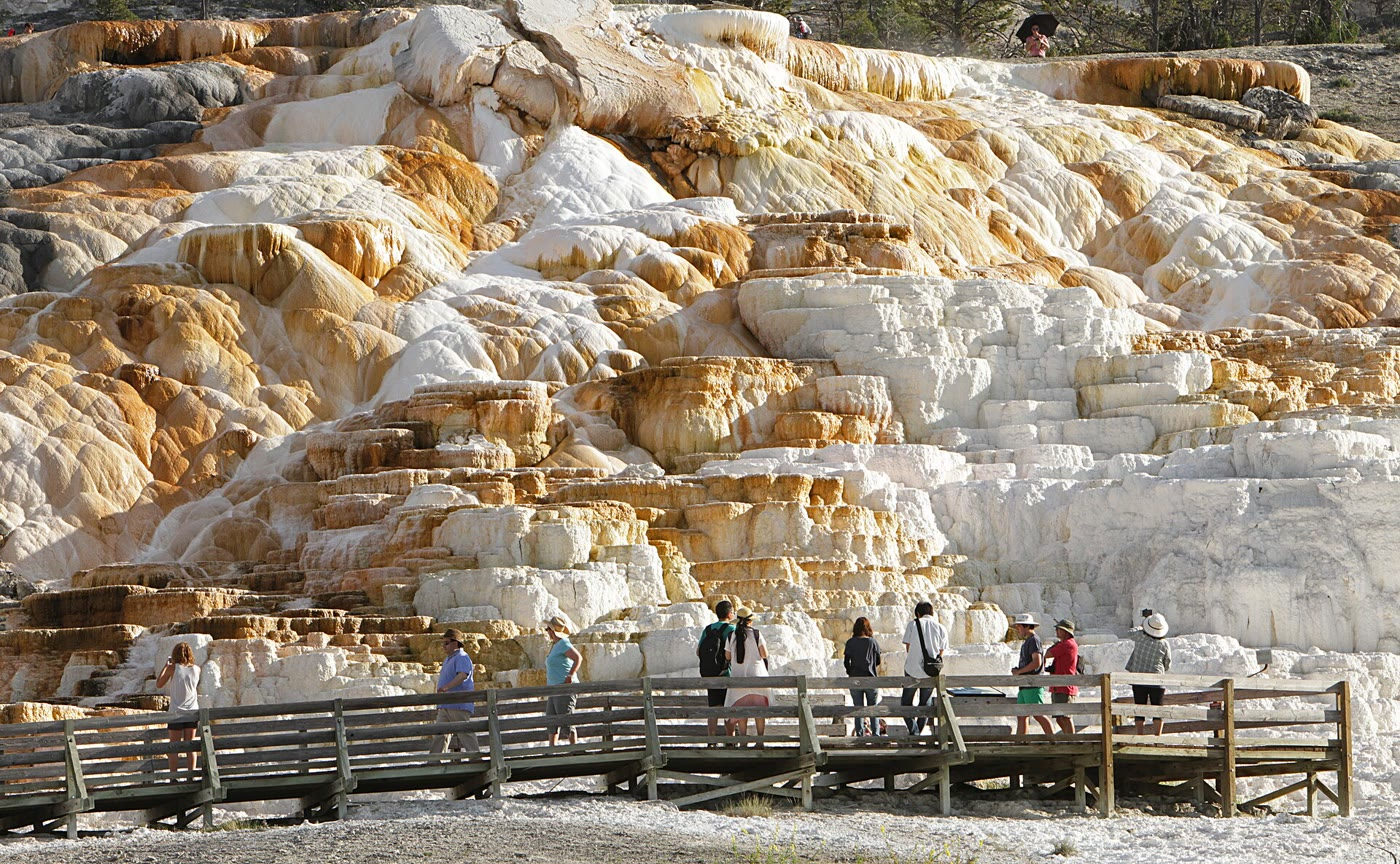
\includegraphics[width=\linewidth]{images/book5/b3-palette-spring-travertine.jpg}

{\scriptsize Terraços de travertino da Palette Spring, Mammoth Hot Springs, com
uma passarela de madeira e visitantes para dar escala. Foto de Jim Peaco, NPS, domínio público.}
\end{minipage}
\end{inthefield}
% ledger: photo:b3-palette-spring, usgsyvo:travertine, nps:travertine-terraces

\section{Cinética do intemperismo de silicatos}\label{sec:b3:water-rock-interaction:kinetics}

Os silicatos se dissolvem muito mais lentamente que a calcita, e uma água raramente atinge o equilíbrio com eles:
sua dissolução precisa ser descrita por uma taxa.

\begin{definition}[Lei de velocidade de dissolução mineral]\label{def:b3:water-rock-interaction:rate-law}
A \emph{lei de velocidade de dissolução mineral}\index{lei de velocidade de dissolução mineral}
fornece a taxa de dissolução por unidade de área superficial do mineral, em
\unit{mol.m^{-2}.s^{-1}}, como uma soma sobre os mecanismos ácido, neutro e básico,
\[
r = \sum_j k_j\,e^{-\frac{E_j}{R}\left(\frac1T - \frac1{298.15}\right)}\,
a_{\ce{H+}}^{n_j}\,\bigl(1 - \Omega^{p_j}\bigr)^{q_j},
\]
com constantes de taxa $k_j$ a \qty{25}{\celsius}, energias de ativação $E_j$,
ordens de reação $n_j$ (negativas para o mecanismo básico) e dois expoentes
$p_j$, $q_j$, geralmente tomados como 1.
\end{definition}
% ledger: pk04:rate-law

\begin{proposition}[Longe e perto do equilíbrio]\label{prop:b3:water-rock-interaction:affinity}
Com $p = q = 1$, a taxa não depende da saturação da água
quando $\Omega \ll 1$, e perto do equilíbrio ela é proporcional ao
índice de saturação: $r \approx -2.303\,r_\infty\,\mathrm{SI}$, em que
$r_\infty$ é a taxa longe do equilíbrio.
\end{proposition}

\begin{proof}
O fator é $1 - \Omega = 1 - 10^{\mathrm{SI}}$. Para $\mathrm{SI} \ll 0$ ele
tende a 1; para $\mathrm{SI}$ próximo de 0, $10^{\mathrm{SI}} \approx 1 +
2.303\,\mathrm{SI}$.
\end{proof}

As constantes de taxa provêm de experimentos de laboratório com pós minerais frescos,
em reatores de fluxo contínuo mantidos longe do equilíbrio. A figura abaixo desenha
a lei de velocidade para quatro minerais a \qty{25}{\celsius}. Cada curva tem a forma de um V ou de um
U: os prótons aceleram a dissolução em água ácida, os íons hidróxido em água básica, e
na faixa intermediária o mecanismo neutro estabelece um patamar mínimo. A olivina se dissolve cerca de três
ordens de grandeza mais rápido que a albita em pH 5, e por isso é o primeiro dos silicatos comuns
a desaparecer de um solo. As energias de ativação da albita e da forsterita,
de 65 a \qty{79}{kJ/mol}, fazem suas taxas quatro a cinco
vezes mais rápidas a \qty{25}{\celsius} do que a \qty{10}{\celsius}.
% ledger: pk04:rates

As taxas de campo são menores, por ordens de grandeza. Em experimentos em colunas com um granito
recém-triturado, a taxa do plagioclásio caiu de forma constante ao longo de seis anos
até \qty{7.0e-14}{mol.m^{-2}.s^{-1}}; o mesmo granito, naturalmente intemperizado,
e em parte transformado em caulinita, dissolveu-se a \qty{2.1e-15}{mol.m^{-2}.s^{-1}}
nas mesmas condições, e ambos ainda são muito mais rápidos que a
taxa medida no próprio perfil de intemperismo. Ao longo de muitos minerais e idades, a
taxa cai com o tempo $t$ em que o mineral vem intemperizando, como $R =
\num{3.1e-13}\,t^{-0.61}$ (mol\,m$^{-2}$\,s$^{-1}$, $t$ em anos). Parte da
queda está no mineral, cujas superfícies mais reativas se dissolvem primeiro; o
restante está no ambiente: água lenta, muito mineral para pouco fluido, e
águas intersticiais próximas do equilíbrio, em que a proposição acima torna a taxa
pequena.
% ledger: whitebrantley03:rates

\begin{omfigure}
\begin{tikzpicture}
\begin{axis}[omrecord, width=0.74\linewidth, height=0.46\linewidth,
  xlabel={pH}, ylabel={$\log r$ (\unit{mol.m^{-2}.s^{-1}})},
  xmin=0, xmax=14, ymin=-14.5, ymax=-6, clip=false,
  xtick={0,2,4,6,8,10,12,14}, ytick={-14,-12,-10,-8,-6},
  yticklabels={$-14$,$-12$,$-10$,$-8$,$-6$},
  tick label style={font=\scriptsize}, label style={font=\small},
  legend style={font=\scriptsize, legend cell align=left, at={(1.03,0.5)}, anchor=west}]
% computed in figdata/bachelor-3/weathering_rates.py
\addplot[green!45!black, thick] table[x=ph, y=forsterite] {figdata/out/bachelor-3-weathering_rates-curves.dat};
\addlegendentry{forsterita}
\addplot[omDef, thick] table[x=ph, y=albite] {figdata/out/bachelor-3-weathering_rates-curves.dat};
\addlegendentry{albita}
\addplot[red!70!black, thick, densely dashed] table[x=ph, y=kfeldspar] {figdata/out/bachelor-3-weathering_rates-curves.dat};
\addlegendentry{feldspato-K}
\addplot[black, thick, densely dotted] table[x=ph, y=kaolinite] {figdata/out/bachelor-3-weathering_rates-curves.dat};
\addlegendentry{caulinita}
\end{axis}
\end{tikzpicture}

\par\smallskip{\small Taxas de dissolução longe do equilíbrio a
\qty{25}{\celsius}, em função do pH, a partir de uma compilação publicada de
parâmetros de taxa de laboratório. O membro extremo olivínico, a forsterita, não tem mecanismo básico na
compilação; sua curva deixa de cair no patamar neutro.}\label{fig:b3:water-rock-interaction:rates}
\end{omfigure}
% ledger: pk04:rates

\begin{definition}[Regimes de intemperismo]\label{def:b3:water-rock-interaction:regimes}
O intemperismo químico numa paisagem está em \emph{regime limitado pelo
suprimento}\index{regime limitado pelo suprimento} quando é limitado pela taxa com que a
erosão traz minerais frescos para a frente de intemperismo, e em
\emph{regime limitado pelo intemperismo}\index{regime limitado pelo intemperismo} quando
os minerais frescos são abundantes e a taxa das reações é que o limita.
\end{definition}

Uma compilação de pequenas bacias de drenagem mostra os dois. Onde a erosão é lenta, sob
solos espessos e lixiviados em relevo suave, o fluxo de intemperismo acompanha a taxa de
erosão: toda rocha fresca que chega é totalmente lixiviada, e um clima mais quente ou
mais úmido pouco altera o resultado. Onde a erosão é rápida, em montanhas íngremes, o
fluxo cresce com o escoamento superficial, como a raiz quadrada da taxa de erosão, e com
a temperatura, com uma energia de ativação aparente de $74 \pm
\qty{29}{kJ/mol}$. Só no segundo regime o intemperismo de silicatos pode atuar como
o termostato climático do volume do segundo ano.
% ledger: west05:regimes

Qual mineral secundário uma água de intemperismo forma é lido em outro
diagrama.

\begin{definition}[Diagrama de atividade]\label{def:b3:water-rock-interaction:activity-diagram}
Um \emph{diagrama de atividade (estabilidade mineral)}\index{diagrama de atividade (estabilidade mineral)}
divide um plano de razões de atividade de uma água, como
$\log(a_{\ce{K+}}/a_{\ce{H+}})$ contra $\log a_{\ce{H4SiO4}}$, nos
campos em que cada mineral de um sistema químico é o estável.
\end{definition}

\begin{proposition}[Limites de um diagrama de atividade]\label{prop:b3:water-rock-interaction:boundaries}
No sistema \ce{K2O}--\ce{Al2O3}--\ce{SiO2}--\ce{H2O}, com alumínio conservado nos sólidos
e água com atividade unitária, um mineral com $k$ átomos de potássio, $a$ de alumínio e
$s$ de silício por fórmula e constante de dissolução $K$ (para \ce{K+},
\ce{Al^3+}, \ce{H4SiO4}) fixa
\[
\log\frac{a_{\ce{Al^3+}}}{a_{\ce{H+}}^3} = \frac{\log K - kX - sY}{a},
\qquad X = \log\frac{a_{\ce{K+}}}{a_{\ce{H+}}},\quad Y = \log a_{\ce{H4SiO4}}.
\]
O mineral estável dá a menor atividade de alumínio, e a fronteira
entre dois minerais é uma reta em $(Y, X)$.
\end{proposition}

\begin{proof}
A dissolução consome $h = k + 3a$ prótons, pelo balanço de cargas, logo $a\log
a_{\ce{Al^3+}} = \log K + h\log a_{\ce{H+}} - k\log a_{\ce{K+}} - s\log
a_{\ce{H4SiO4}}$; dividindo por $a$ e passando $3\log a_{\ce{H+}}$ para a esquerda
obtém-se a expressão. Uma água em equilíbrio com um mineral está
subsaturada em relação a qualquer mineral que exigiria mais alumínio, e
supersaturada em relação a qualquer um que exigiria menos; logo, o menos solúvel é
o estável. Igualando duas dessas expressões, lineares em $X$ e $Y$, obtém-se uma reta.
\end{proof}

Com as constantes a \qty{25}{\celsius}, a gibbsita cede lugar à caulinita em
$\log a_{\ce{H4SiO4}} = -4.39$ (\qty{2.4}{mg/L} de sílica) e a caulinita cede lugar à
muscovita em $\log(a_{\ce{K+}}/a_{\ce{H+}}) = 1.55$, e o feldspato-K é estável
apenas em águas ricas em potássio e sílica. O diagrama é a sequência de intemperismo
do volume do primeiro ano expressa em números: uma água diluída que lixivia
o potássio e a sílica desgasta um feldspato até a gibbsita; uma água que
retém mais sílica forma caulinita; uma que retém mais potássio, como em profundidade,
forma uma mica.
% ledger: phreeqc:silicates

\begin{omfigure}
\begin{tikzpicture}
\begin{axis}[omrecord, width=0.66\linewidth, height=0.5\linewidth,
  xlabel={$\log a_{\ce{H4SiO4}}$}, ylabel={$\log(a_{\ce{K+}}/a_{\ce{H+}})$},
  xmin=-6, xmax=-2, ymin=0, ymax=10, clip=false,
  xtick={-6,-5,-4,-3,-2}, xticklabels={$-6$,$-5$,$-4$,$-3$,$-2$},
  tick label style={font=\scriptsize}, label style={font=\small}]
% computed in figdata/bachelor-3/activity_diagram.py
\addplot[black, thick, unbounded coords=jump] table[x=y, y=x] {figdata/out/bachelor-3-activity_diagram-lines.dat};
\addplot[omDef, densely dashed] table[x=y, y=x] {figdata/out/bachelor-3-activity_diagram-quartz.dat};
\addplot[omDef, densely dotted] table[x=y, y=x] {figdata/out/bachelor-3-activity_diagram-amorph.dat};
\addplot[red!70!black, only marks, mark=*, mark size=1.8pt] table[x=y, y=x] {figdata/out/bachelor-3-activity_diagram-samples.dat};
\node[font=\small] at (axis cs:-5.4,0.8) {gibbsita};
\node[font=\small] at (axis cs:-3.25,0.75) {caulinita};
\node[font=\small] at (axis cs:-4.6,5.0) {muscovita};
\node[font=\small] at (axis cs:-3.3,9.3) {feldspato-K};
\node[font=\scriptsize, omDef, anchor=south] at (axis cs:-3.98,10) {quartzo};
\node[font=\scriptsize, omDef, anchor=south] at (axis cs:-2.71,10) {sílica amorfa};
\node[font=\scriptsize, red!70!black, anchor=west] at (axis cs:-4.58,0.38) {A};
\node[font=\scriptsize, red!70!black, anchor=west] at (axis cs:-3.80,1.29) {B};
\node[font=\scriptsize, red!70!black, anchor=west] at (axis cs:-3.48,4.08) {C};
\end{axis}
\end{tikzpicture}

\par\smallskip{\small Campos de estabilidade no sistema
\ce{K2O}--\ce{Al2O3}--\ce{SiO2}--\ce{H2O} a \qty{25}{\celsius}, com a saturação de quartzo
(tracejado) e de sílica amorfa (pontilhado). Três águas inventadas: A, um riacho tropical
diluído; B, um riacho sobre granito; C, uma água subterrânea profunda em
granito.}\label{fig:b3:water-rock-interaction:activity}
\end{omfigure}
% ledger: phreeqc:silicates

\section{Fluidos hidrotermais}\label{sec:b3:water-rock-interaction:hydrothermal}

Água quente que circula pela crosta, perto de uma dorsal ou de uma intrusão,
troca oxigênio com a rocha que atravessa. Em alta temperatura o
fracionamento entre rocha e água é pequeno, e ambos tendem
ao equilíbrio isotópico: a água meteórica, leve, torna a rocha mais leve, e a
água, mais pesada. Quanto a rocha se deslocou mede quanta água
passou.

\begin{definition}[Razão água--rocha]\label{def:b3:water-rock-interaction:water-rock-ratio}
A \emph{razão água--rocha}\index{razão água--rocha} $W/R$ de um
sistema hidrotermal é a massa de água que trocou com uma massa de
rocha, dividida por essa massa de rocha.
\end{definition}

\begin{proposition}[Razões água--rocha a partir de isótopos de oxigênio]\label{prop:b3:water-rock-interaction:wr}
Seja uma rocha de $\delta_r^i$ inicial que troca oxigênio com uma água de
$\delta_w^i$ inicial até atingir $\delta_r^f$, em equilíbrio com a água com que
esteve por último, $\Delta = \delta_r^f - \delta_w^f$, e sejam $c_r$ e $c_w$
as concentrações de oxigênio da rocha e da água. Num sistema fechado (um lote de
água) e num aberto (água que passa uma única vez),
\[
\frac WR\Big|_{\text{fechado}} = \frac{c_r}{c_w}\,
\frac{\delta_r^f - \delta_r^i}{\delta_w^i - \delta_r^f + \Delta},
\qquad
\frac WR\Big|_{\text{aberto}} = \frac{c_r}{c_w}\,
\ln\!\left(\frac{\delta_r^f - \delta_r^i}{\delta_w^i - \delta_r^f + \Delta} + 1\right).
\]
\end{proposition}

\begin{proof}
Fechado: o oxigênio-18 se conserva, $c_wW\delta_w^i + c_rR\delta_r^i = c_wW
\delta_w^f + c_rR\delta_r^f$, com $\delta_w^f = \delta_r^f - \Delta$; isola-se
$W/R$. Aberto: uma porção $\mathrm dW$ entra com $\delta_w^i$ e sai em
equilíbrio com a rocha, em $\delta_r - \Delta$, de modo que $c_rR\,\mathrm d\delta_r
= c_w(\delta_w^i - \delta_r + \Delta)\,\mathrm dW$. Separando as variáveis,
$\int_{\delta_r^i}^{\delta_r^f}\mathrm d\delta_r/(\delta_w^i - \delta_r +
\Delta) = (c_w/c_r)\,W/R$, e a integral vale $-\ln[(\delta_w^i - \delta_r^f
+ \Delta)/(\delta_w^i - \delta_r^i + \Delta)]$, que é a expressão.
\end{proof}

Para o oxigênio, $c_r/c_w$ fica próximo de 0.5. O sistema aberto sempre precisa
de menos água do que o fechado para a mesma variação, porque cada porção sai
tão pesada quanto pode. Em torno de muitas intrusões, o $\delta^{18}\mathrm O$
da rocha encaixante desenha um alvo de valores baixos, de cerca de $+6$ até
abaixo de 0, centrado onde passou a maior quantidade de água; os minérios do
fluido hidrotermal costumam estar dentro do contorno mais baixo, o que torna o
mapa uma ferramenta de prospecção.
% ledger: white13c9:water-rock

\begin{omfigure}
\begin{tikzpicture}[font=\small, >=Stealth]
\draw[thick, fill=black!6] (0,0) rectangle (4,2.2);
\node at (2,1.55) {rocha, massa $R$};
\node at (2,0.95) {$\delta_r^i \to \delta_r^f$};
\node[font=\scriptsize] at (2,0.4) {troca à temperatura $T$};
\draw[->, thick, omDef] (-2.6,1.1) -- (-0.1,1.1);
\node[omDef, anchor=south, align=center, font=\scriptsize] at (-1.35,1.15) {água entra\\ $\delta_w^i$, $\mathrm dW$};
\draw[->, thick, red!70!black] (4.1,1.1) -- (6.6,1.1);
\node[red!70!black, anchor=south, align=center, font=\scriptsize] at (5.35,1.15) {água sai\\ $\delta_r - \Delta$};
\node[anchor=north, font=\scriptsize, align=center] at (2,-0.15) {sistema aberto: cada porção passa uma vez e sai em\\ equilíbrio com a rocha que encontrou por último};
\end{tikzpicture}

\par\smallskip{\small O modelo de caixas de um sistema hidrotermal. Em um
sistema fechado, um lote de água permanece com a rocha até que ambas estejam
em equilíbrio; em um sistema aberto, a água flui através da rocha, e esta se
desloca um pouco em direção à água a cada porção.}\label{fig:b3:water-rock-interaction:box}
\end{omfigure}

\begin{definition}[Modelo de trajetória de reação]\label{def:b3:water-rock-interaction:reaction-path}
Um \emph{modelo de trajetória de reação}\index{modelo de trajetória de reação} acompanha a composição
de uma água e os minerais que ela forma à medida que a reação avança, acrescentando pequenas
quantidades de um reagente (um mineral se dissolvendo, um gás escapando, calor sendo retirado) e
recalculando a especiação e os índices de saturação a cada etapa,
precipitando qualquer mineral que atinja a saturação.
\end{definition}

Um \omterm{def:b3:water-rock-interaction:reaction-path}{modelo de trajetória de reação} aplicado à nascente do problema de fim de
semana, com desgaseificação passo a passo, precipita calcita assim que o seu
índice ultrapassa zero; aplicado a um granito e a uma água de chuva, ele forma
gibbsita primeiro, depois caulinita, depois mica à medida que a água acumula
sílica e potássio, traçando uma trajetória no diagrama de atividade. Programas
de especiação fazem isso com bancos de dados de constantes de equilíbrio como os usados neste capítulo.
% ledger: phreeqc:silicates

\section{Exercícios}

\begin{exercise}[$\star$]\label{exo:b3:water-rock-interaction:1}
Uma água tem (em \unit{mg/L}) \ce{Ca} 48, \ce{Mg} 9.7, \ce{Na} 23, \ce{K} 3.9,
\ce{HCO3} 183, \ce{Cl} 35.5 e \ce{SO4} 48. Calcule o erro de balanço de
cargas. A análise é aceitável?
\end{exercise}

\begin{exercise}[$\star$]\label{exo:b3:water-rock-interaction:2}
Para uma força iônica de 0.0050, calcule os coeficientes de atividade de
\ce{Ca^2+}, \ce{HCO3-} e \ce{SO4^2-}.
\end{exercise}

\begin{exercise}[$\star$]\label{exo:b3:water-rock-interaction:3}
Uma água que drena uma marga com gipsita contém \qty{3.0}{mmol/L} de cálcio e
\qty{4.0}{mmol/L} de sulfato, com força iônica de 0.016. Calcule o índice de
saturação da gipsita. A água ainda pode dissolver gipsita?
\end{exercise}

\begin{exercise}[$\star$]\label{exo:b3:water-rock-interaction:4}
Uma água subterrânea contém \qty{12}{mg/L} de sílica, expressa como \ce{SiO2} e
presente como \ce{H4SiO4}. Calcule seus índices de saturação para o quartzo e
para a sílica amorfa a \qty{25}{\celsius}.
\end{exercise}
% ledger: phreeqc:silicates

\begin{exercise}[$\star\star$]\label{exo:b3:water-rock-interaction:5}
Considerando os coeficientes de atividade iguais a 1, calcule o cálcio dissolvido
por um sistema aberto a $P_{\ce{CO2}} = 10^{-2}$~atm a \qty{25}{\celsius} e a
\qty{10}{\celsius}, em \unit{mmol/L} e \unit{mg/L}.
\end{exercise}

\begin{exercise}[$\star\star$]\label{exo:b3:water-rock-interaction:6}
Uma água a \qty{25}{\celsius} tem pH 7.60 e \qty{4.0}{mmol/L} de bicarbonato.
Com coeficientes de atividade iguais a 1, calcule seu dióxido de carbono dissolvido
e seu carbonato, sua $P_{\ce{CO2}}$ e a fração de cada espécie no
carbono inorgânico dissolvido.
\end{exercise}

\begin{exercise}[$\star\star$]\label{exo:b3:water-rock-interaction:7}
Um grão de albita é uma esfera de \qty{1}{mm} de diâmetro em uma água de solo
de pH 5 a \qty{25}{\celsius}, dissolvendo-se à taxa da figura, $\log r = -12.09$.
Com um volume molar de \qty{101.31}{cm^3/mol}, com que rapidez o seu raio
diminui, e quanto tempo dura o processo?
\end{exercise}
% ledger: pk04:rates, phreeqc:silicates

\begin{exercise}[$\star\star$]\label{exo:b3:water-rock-interaction:8}
Por qual fator a taxa de dissolução neutra da albita ($E =
\qty{69.8}{kJ/mol}$) cresce de \qty{5}{\celsius} para \qty{25}{\celsius}? E
um fluxo de intemperismo com $E = \qty{74}{kJ/mol}$?
\end{exercise}
% ledger: pk04:rates, west05:regimes

\begin{exercise}[$\star\star$]\label{exo:b3:water-rock-interaction:9}
Derive a fronteira caulinita--muscovita do diagrama de atividade a partir das
constantes $\log K = 7.435$ (caulinita, 2 Al, 2 Si) e $12.703$ (muscovita, 1
K, 3 Al, 3 Si). Uma água a \qty{25}{\celsius} tem \qty{2.0}{mg/L} de potássio,
\qty{15}{mg/L} de sílica e pH 7.0: qual mineral ela forma?
\end{exercise}
% ledger: phreeqc:silicates

\begin{exercise}[$\star\star\star$]\label{exo:b3:water-rock-interaction:10}
Perto de uma intrusão, um granodiorito de $\delta^{18}\mathrm O = +6$
fica em $-2$ (\unit{\permil}). A água meteórica tinha $-13$, e na temperatura
de troca a rocha era \qty{2}{\permil} mais pesada que a água. Com $c_r/c_w = 0.5$,
calcule a \omterm{def:b3:water-rock-interaction:water-rock-ratio}{razão água--rocha} para um sistema fechado e
para um sistema aberto, e explique por que elas diferem.
\end{exercise}
% ledger: white13c9:water-rock

\begin{exercise}[$\star\star\star$]\label{exo:b3:water-rock-interaction:11}
Chuva carregada com gás do solo, com $P_{\ce{CO2}} = 10^{-1.5}$~atm a
\qty{10}{\celsius} atinge um calcário. Com coeficientes de atividade iguais a 1,
calcule o cálcio que ela dissolve se permanecer aberta ao gás do solo e se for
isolada dele antes. Qual fração do seu dióxido de carbono resta no
caso fechado, e qual é a $P_{\ce{CO2}}$ final?
\end{exercise}

\begin{exercise}[$\star\star\star$]\label{exo:b3:water-rock-interaction:12}
Usando a proposição sobre taxas próximas do equilíbrio, qual fração da sua
taxa longe do equilíbrio um mineral se dissolve com $\mathrm{SI} =
-2$, $-1$ e $-0.1$? Uma taxa de laboratório medida após 6 anos de reação
segue a lei de potência do capítulo: por qual fator ela terá caído
após \num{10000}~anos? Combine os dois efeitos para explicar por que as taxas de campo são
tão baixas.
\end{exercise}
% ledger: whitebrantley03:rates

\section{Problema: a nascente abaixo do calcário Varden}

\begin{problem}[{Problema de fim de semana --- a análise, o dióxido de carbono e
a saturação de uma nascente de calcário inventada, e um riacho de granito}]
\label{pb:b3:water-rock-interaction:1}
Uma nascente surge ao pé do calcário jurássico das colinas Varden, a
\qty{10}{\celsius} e pH 7.20. Sua análise é (em \unit{mg/L}): \ce{Ca}
112, \ce{Mg} 4.0, \ce{Na} 7.0, \ce{K} 1.2, \ce{HCO3} 340, \ce{Cl} 11,
\ce{SO4} 14, \ce{NO3} 9. A \qty{10}{\celsius}: $\log K_{\mathrm{cal}} =
-8.35$, $\log K_1 = -6.46$, $\log K_2 = -10.49$, $\log K_H = -1.27$. Use a
equação de Debye--Hückel estendida do capítulo, ignore pares iônicos e tome
o ar com $\log P_{\ce{CO2}} = -3.37$.

\medskip\noindent\textbf{Parte I --- A análise.}
\begin{enumerate}
\item Converta a análise para \unit{mmol/L}.
\item Calcule o erro de balanço de cargas. A análise é aceitável?
\item Calcule a força iônica.
\item Calcule os coeficientes de atividade de \ce{Ca^2+}, \ce{HCO3-} e
  \ce{CO3^2-}.
\item A equação de Debye--Hückel estendida é válida aqui?
\end{enumerate}

\medskip\noindent\textbf{Parte II --- Dióxido de carbono.}
\begin{enumerate}[resume]
\item Calcule a atividade do bicarbonato.
\item Calcule a atividade do dióxido de carbono dissolvido.
\item Calcule a $P_{\ce{CO2}}$ da nascente. Quantas vezes ela é maior que a
  do ar, e de onde pode vir o dióxido de carbono?
\item Calcule a concentração de carbonato e a participação de cada espécie no
  carbono inorgânico dissolvido.
\item Verifique que a alcalinidade é quase toda bicarbonato.
\end{enumerate}

\medskip\noindent\textbf{Parte III --- Saturação e travertino.}
\begin{enumerate}[resume]
\item Calcule o produto de atividade iônica e o índice de saturação da calcita
  na saída.
\item A nascente está em equilíbrio com a calcita? É uma nascente de conduto ou
  uma nascente lenta e difusa?
\item Calcule o cálcio de um sistema aberto em equilíbrio com a calcita na
  $P_{\ce{CO2}}$ da nascente, com os coeficientes de atividade da questão 4,
  e compare com a análise.
\item A água desgaseifica para o ar antes que se forme qualquer calcita. Mantendo a
  atividade do bicarbonato inalterada, calcule seu pH e seu índice de saturação.
\item Estime o cálcio que ela mantém depois de ter precipitado calcita até voltar
  ao equilíbrio com o ar (sistema aberto, coeficientes de atividade na nova
  força iônica $3m$), e a massa de calcita por litro.
\item A nascente escoa a \qty{2.0}{L/s} e espalha seu depósito por
  \qty{400}{m^2}. Se toda essa calcita permanecesse ali, com densidade de
  \qty{2.71}{g/cm^3}, com que rapidez o depósito cresceria?
\end{enumerate}

\medskip\noindent\textbf{Parte IV --- O riacho de granito.} Um riacho sobre o
granito Varden, sob um solo espesso em encostas suaves, tem (a
  \qty{25}{\celsius}) \qty{1.2}{mg/L} de potássio, \qty{9.0}{mg/L} de
  sílica e pH 5.8.
\begin{enumerate}[resume]
\item Calcule sua posição no diagrama de atividade.
\item Qual mineral ele forma? Calcule seu índice de saturação para o quartzo.
\item Abaixo de qual concentração de sílica ele formaria gibbsita?
\item Em qual pH ele atingiria a fronteira caulinita--muscovita?
\item Calcule a taxa de dissolução do feldspato-K nessa água, longe do
  equilíbrio, a partir dos parâmetros $\log k = -10.06$, $n = 0.500$ (ácido);
  $-12.41$ (neutro); $-21.20$, $n = -0.823$ (básico).
\item O intemperismo desta bacia é mais provavelmente limitado pelo suprimento ou
  limitado pelo intemperismo? Por quê?
\item Com uma energia de ativação aparente de \qty{74}{kJ/mol}, por qual fator
  um fluxo limitado pelo intemperismo mudaria entre \qty{10}{\celsius} e
  \qty{25}{\celsius}?
\item Informe o índice de saturação da calcita da água da nascente em sua
  saída.
\end{enumerate}
\end{problem}
% ledger: phreeqc:carbonate, phreeqc:silicates, hem85:debye-huckel, hem85:charge-balance, hem85:si, hem85:pco2, pk04:rates, west05:regimes, data:co2-mlo
